\section{Mission Planning}
For UAV, the autonomy is characterized by its level of
interaction with the operator: the more abstract the operator decisions are, the more autonomous the vehicle is. Mission planning and flight scheduling, computing an appropriate path for the vehicle in order to achieve the objectives of the mission, is one of the main challenges for UAV development in order to increase the autonomy level. Usually, mission planning is used to describe all these tasks\cite{4281723}

The first step in the design is to decide on the scales or its resolution and the requirement accuracy. Once those two requirement are know, the following processes follow:
\begin{enumerate}
\item Planning the aerial photography (developing the flight plan);
\item Planning the ground controls;
\item Selecting software, instruments and procedures necessary to produce the final products
\end{enumerate}
For the flight plan, the planner needs to know the following information, some of which are computed.\cite{Design_plann}
\begin{itemize}
\item The amount of end lap and side lap.
\item Flying height.
\item Focal length of the camera lens.
\item Size of the CCD.
\item Size of CCD Array (how many pixels).
\item Size and shape of the area to be photographed.
\item Ground speed of aircraft.
\end{itemize}.

\subsection{Front and over lap}
When an area is covered by vertical aerial photography, the photographs are usually taken along a series of parallel passes, called \textit{flight strips}. As shown in figure \ref{fig:EndLap}, the photographs are normally exposed in such way that the area covered by each successive photograph along a flight strip duplicates or overlaps part of the ground of previous photo. This is lapping along the flight strip is called \textit{end lap}, and the area coverage common to to an adjacent pair of photographs in a flight strip is called the \textit{stereoscopic overlap area}. the overlapping pair of photo is called \textit{stereopair}\cite{elements_photogrammetry}.
\begin{figure}[H]
\centering
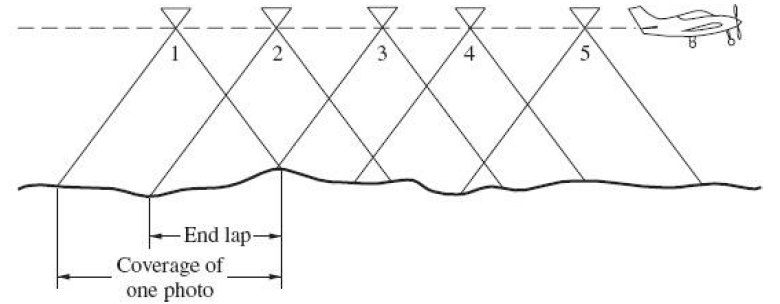
\includegraphics[width=10cm,height=10cm,keepaspectratio]{imagenes/EndLap.PNG}
\caption{End lap of photographs in a flight strip}
\label{fig:EndLap}
\end{figure}
Adjacent flight strips area photograph so that there is also a lateral overlapping of ground coverage between strips. This condition shown in figure \ref{fig:SideLap}, is called \textit{side lap}\cite{elements_photogrammetry}.
\begin{figure}[H]
\centering
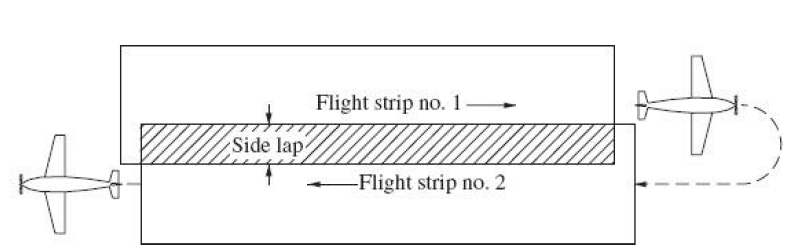
\includegraphics[width=10cm,height=10cm,keepaspectratio]{imagenes/sidelap.PNG}
\caption{Side lap of adjacent flight strips}
\label{fig:SideLap}
\end{figure}

\subsection{Flying height computation}
The flight height H that is need to obtain a given GSD can be computed and depends on the camera focal length, the camera sensor width  (mm), and the image width (pixels).\cite{GSDComputation}
\begin{figure}[H]
\centering
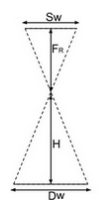
\includegraphics[width=4cm,height=4cm,keepaspectratio]{imagenes/GSD.PNG}
\caption{GSD variable definition}
\label{fig:GSD}
\end{figure}
\begin{table}[H]
\centering
\begin{tabular}{|c|c|}
\hline
\textbf{Variable} & \textbf{Definition}                                                                      \\ \hline
Sw                & Real sensor width (mm)                                                                   \\ \hline
FR                & Real Focal length (mm)                                                                   \\ \hline
H                 & Flight height (m)                                                                        \\ \hline
Dw                & Distance covered on the ground by one image (footprint width) (m) \\ \hline
\end{tabular}
\caption{GSD variable definition}
\end{table}
Using the fact that:
\begin{equation}
H/F_{R} = D_{w}/S_{w}
\end{equation}
The flight height H is given by:
\begin{equation}
H = (D_{W}\cdot F_{R})/S_{W}
\label{H}
\end{equation}
The distance covered on the ground by one image in the width direction (foot print width) is given by:
\begin{equation}
D_{w}=(imW*GSD)/100
\label{DW}
\end{equation}
\begin{table}[H]
\centering
\begin{tabular}{|c|c|}
\hline
\textbf{Variable} & \textbf{Definition}   \\ \hline
imW              & Image width (pixels)  \\ \hline
GSD               & Desire GSD (cm/pixel) \\ \hline
\end{tabular}
\caption{Height equation Variable definition}
\end{table}
Combining equations \ref{H} and \ref{DW}, the flight height is given by:
\begin{equation}
H[m]=(imW\cdot GSD \cdot F_{R})\cdot (S_{w}*100)
\end{equation}
Image shotting rate to achieve a given overlap depends on the speed of the UAS, the GSD and the pixel resolution of the camera.
\begin{table}[H]
\centering
\begin{tabular}{|c|c|}
\hline
Variable & Definition                                                                  \\ \hline
D        & Distance covered on the ground by one image in the flight direction {[}m{]} \\ \hline
Overlap  & percentage of desire frontal overlap between two images.                    \\ \hline
X        & Distance between two images in the flight direction. {[}m{]}                \\ \hline
V        & flight speed {[}m/s{]}                                                      \\ \hline
t        & elapsed time between two images (image rate) {[}s{]}                        \\ \hline
imH      & Image height {[}pixel{]}                                                    \\ \hline
\end{tabular}
\caption{Time equation variable definition}
\end{table}
\begin{figure}[H]
\centering
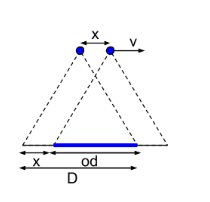
\includegraphics[width=6cm,height=6cm,keepaspectratio]{imagenes/velocity.PNG}
\caption{Velocity computing variables}
\label{fig:velocity}
\end{figure}
form figure \ref{fig:velocity}, we obtain the following equations:
\begin{equation}
od =overlap\cdot D
\label{od}
\end{equation}
\begin{equation}
x=D\cdot od
\label{x}
\end{equation}
\begin{equation}
t = x/v
\label{t}
\end{equation}
\begin{equation}
D=D_{h}=(imH\cdot GSD)/100
\label{D}
\end{equation}
Combining equations: \ref{od} and \ref{D} into equation \ref{x}:
\begin{equation}
x = D_{h}-overlap\cdot D_{h}
\end{equation}
\begin{equation}
x= D_{h\cdot (1-overlap)}
\end{equation}
\begin{equation}
x = ((imH\cdot GSD)/100)\cdot (1-overlap)
\label{X_large}
\end{equation}
Combing the equations \ref{t} and \ref{X_large}:
\begin{equation}
t=x/v=\frac{((imH\cdot GSD)/100)\cdot (1-overlap)}{v}
\end{equation}
\subsection{Flight path design}
For a rectangularly shaped project, always use the smallest dimension of the project area to layout your flight lines. This way it results in fewer flight lines and then less turns between flight lines. In Figure \ref{fig:line_orientaion}, the red lines with arrowheads represent flight lines or strips, while the black dash lines represent the project boundary.
\begin{figure}[H]
\centering
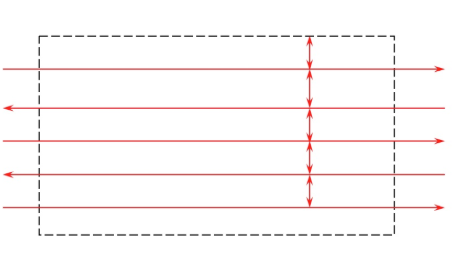
\includegraphics[width=10cm,height=10cm,keepaspectratio]{imagenes/flight_path.PNG}
\caption{Correct flight lines orientation}
\label{fig:line_orientaion}
\end{figure}
If you have a digital camera with a rectangular shape CCD array, always choose the largest dimension of the CCD array of the camera to be perpendicular to the flight direction. In Figure \ref{fig:camera_orientaion}, the blue rectangles represent images as taken by a camera with rectangular CCD array. The wider dimension of the array is always configured to be perpendicular to the flight direction\cite{GCP}
\begin{figure}[H]
\centering
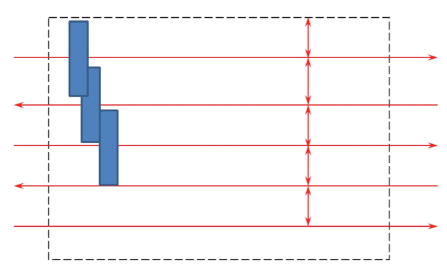
\includegraphics[width=10cm,height=10cm,keepaspectratio]{imagenes/flight_path_oritentation.PNG}
\caption{Correct camera orientation}
\label{fig:camera_orientaion}
\end{figure}
\begin{table}[H]
\centering
\begin{tabular}{|c|c|}
\hline
\textbf{Variable} & \textbf{Definition}                           \\ \hline
SP                & Line spacing or distance between flight lines \\ \hline
D                 & Image coverage                                \\ \hline
SL                & Amount of side lap                            \\ \hline
NFL               & Number of flight lines                        \\ \hline
\end{tabular}
\label{Flight line amount equation variable definition}
\end{table}
To procedure to compute the number of flight lines is shown in the following procedure.
\begin{enumerate}
\item Compute the coverage on the ground of one image using equation \ref{D}
\item Compute the flight lines spacing as follows:
\begin{equation}
SP = D\cdot \frac{(100-SL)}{100}
\end{equation}
\item Number of flight lines (NFL) is computed as follow:
\begin{equation}
NFL=\frac{width}{SP}+1
\end{equation}
\end{enumerate}
\begin{figure}[H]
\centering
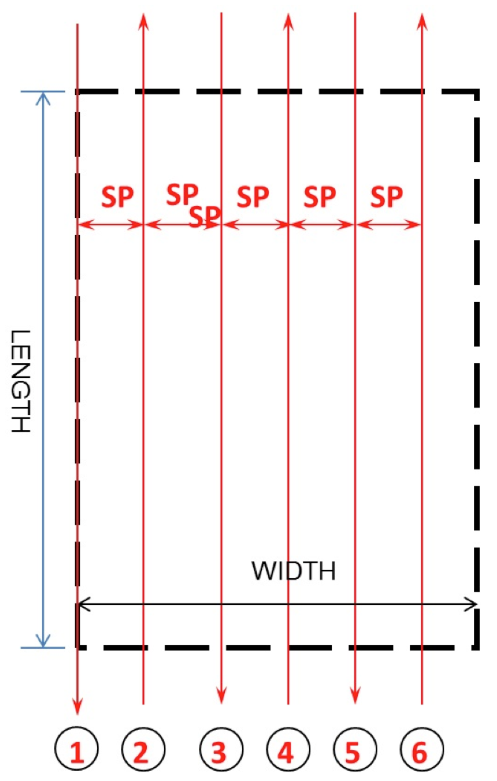
\includegraphics[width=10cm,height=10cm,keepaspectratio]{imagenes/flight_lines.PNG}
\caption {Flight line layouts}
\label{fig:flight_lines}
\end{figure}

\subsection{Poly survey}
The poly survey is a navigation routine, that the aircraft follows to survey the area of any convex polygon given an entry point, the number of waypoints which define the polygon, the sweep width and the desired orientation of the sweeps.
\begin{figure}[H]
\centering
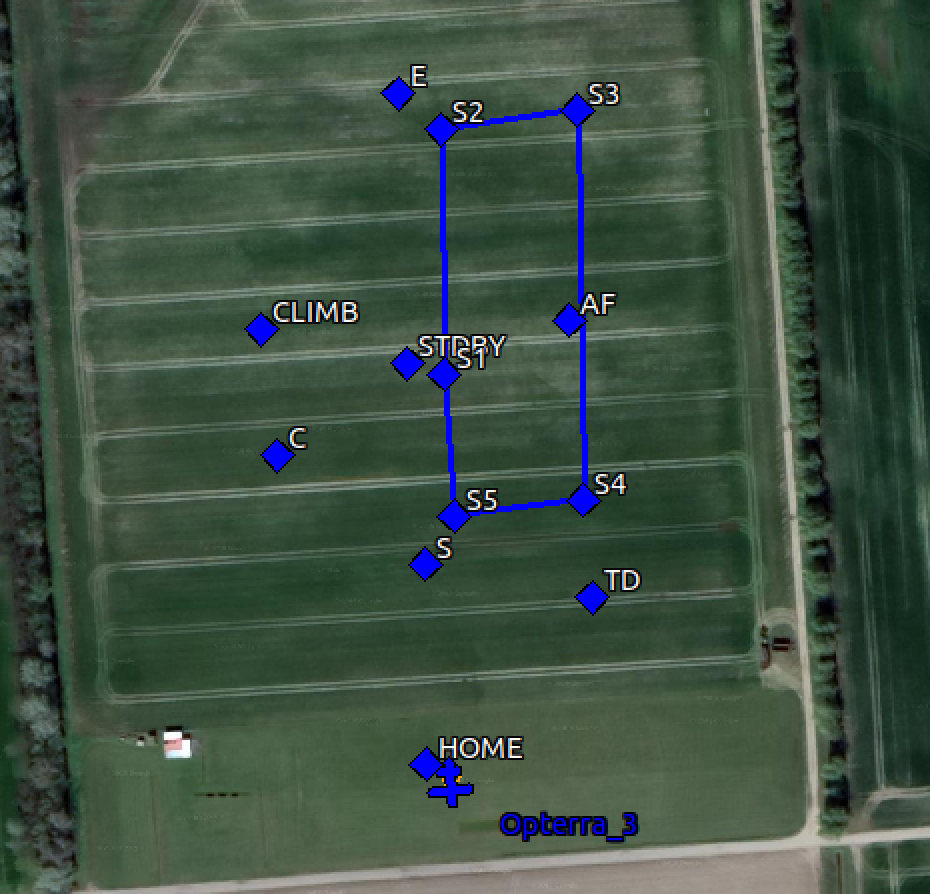
\includegraphics[width=10cm,height=10cm,keepaspectratio]{imagenes/Convex_polygon.png}
\caption{Example of a poly survey convex polygon}
\label{fig:Convex_poly}
\end{figure}
The entry point is the first corner of the polygon and the point at which the aircraft will begin surveying the area. When in the entry state, the aircraft will circle around the entry point in order to smoothly transition into the first sweep. The aircraft will also keep circling around the entry point until it gets to the waypoint altitude. After the first sweep is made, the direction of the next sweep is determined by the distance of the entry point to the edges of the polygon. If there is more area above the first sweep, the aircraft will sweep up. If there is more area below the first sweep, the aircraft will sweep down.\cite{Poly_survey}

The aircraft will keep sweeping back and forth until it reaches the end of the polygon. At this point, the aircraft will sweep back up/down the polygon halfway in between the sweeps previously made by the aircraft. 
\begin{figure}[H]
\centering
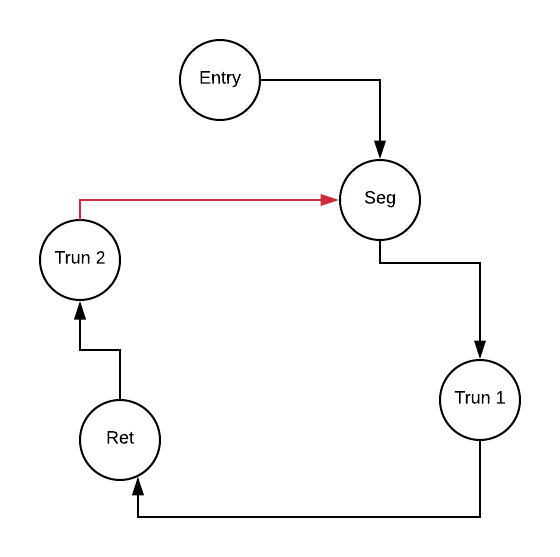
\includegraphics[width=10cm,height=10cm,keepaspectratio]{imagenes/FSM.png}
\caption{Poly survey Finite state machine }
\label{fig:FSM}
\end{figure}

The poly survey algorithm is a multistage finite state machine consisting of five different stages: Entry, Seg, Turn, Ret and Turn 2.
\subsubsection{Entry}
The first task performed \textit{Entry} is to compute the value of space between lines, numbers of lines and distance between photos, utilizing the equation stated above.  Having these values the algorithms will guide the plane to a circle a point near the entry waypoint until it reaches the desired altitude. As seen in the image \ref{fig:entry_stage}, The plane is climbing while flying in a circle near the entry waypoint WP1
\begin{figure}[H]
\centering
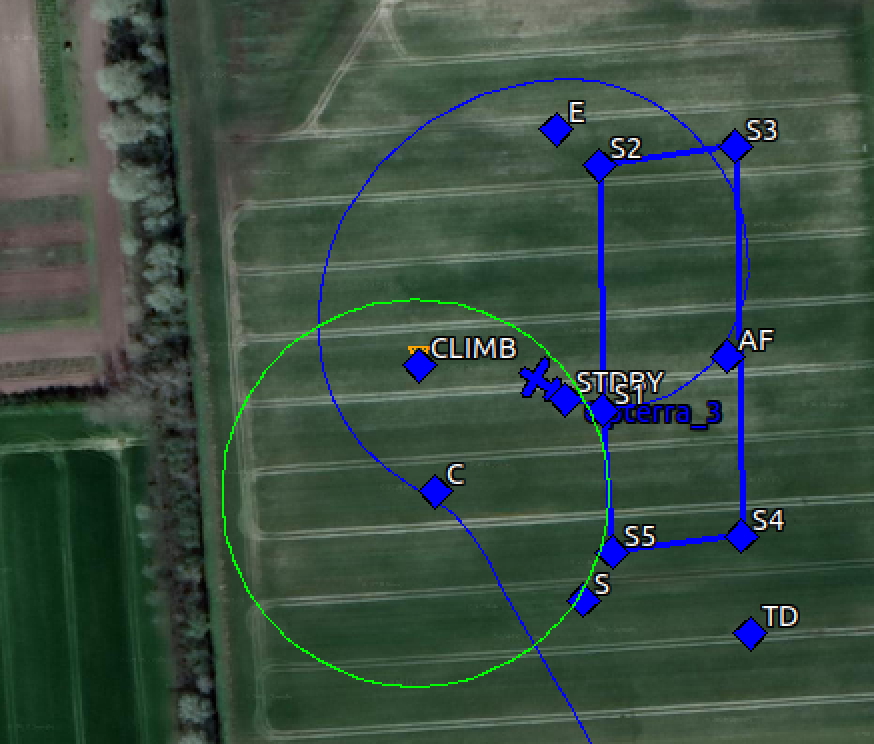
\includegraphics[width=10cm,height=10cm,keepaspectratio]{imagenes/Entry.png}
\caption{Simulation of poly survey, entry stage}
\label{fig:entry_stage}
\end{figure}
If the altitude, position, and orientation of the plane are correct the FMS will change to \textit{Seg}. Before the transition to Seg, the camera will start taking photos with the distance interval that was computed earlier.
\subsubsection{Seg}
\textit{Seg} is the state where the plane will survey the area under study. The plane will follow a straight line taking photos until it will reach the end of the segment. At that point, the plain will automatically stop taking photos and save them on the memory of the camera and transition to Turn 1.
\begin{figure}[H]
\centering
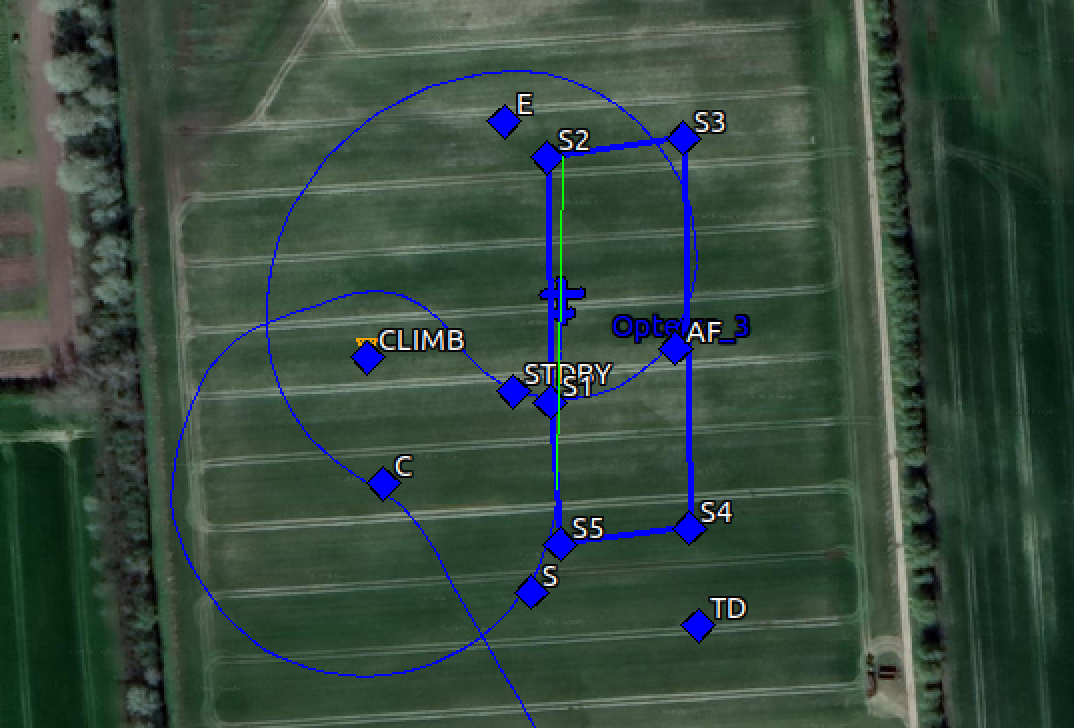
\includegraphics[width=10cm,height=10cm,keepaspectratio]{imagenes/SEG.png}
\caption{Simulation of poly survey, SEG stage}
\label{fig:SEG_stage}
\end{figure}

In figure \ref{fig:SEG_stage} the plane is following a straight segment while taking photos. Figure \ref{fig:Photos}, shows a simulation of the photos taken by the camera.
\begin{figure}[H]
\centering
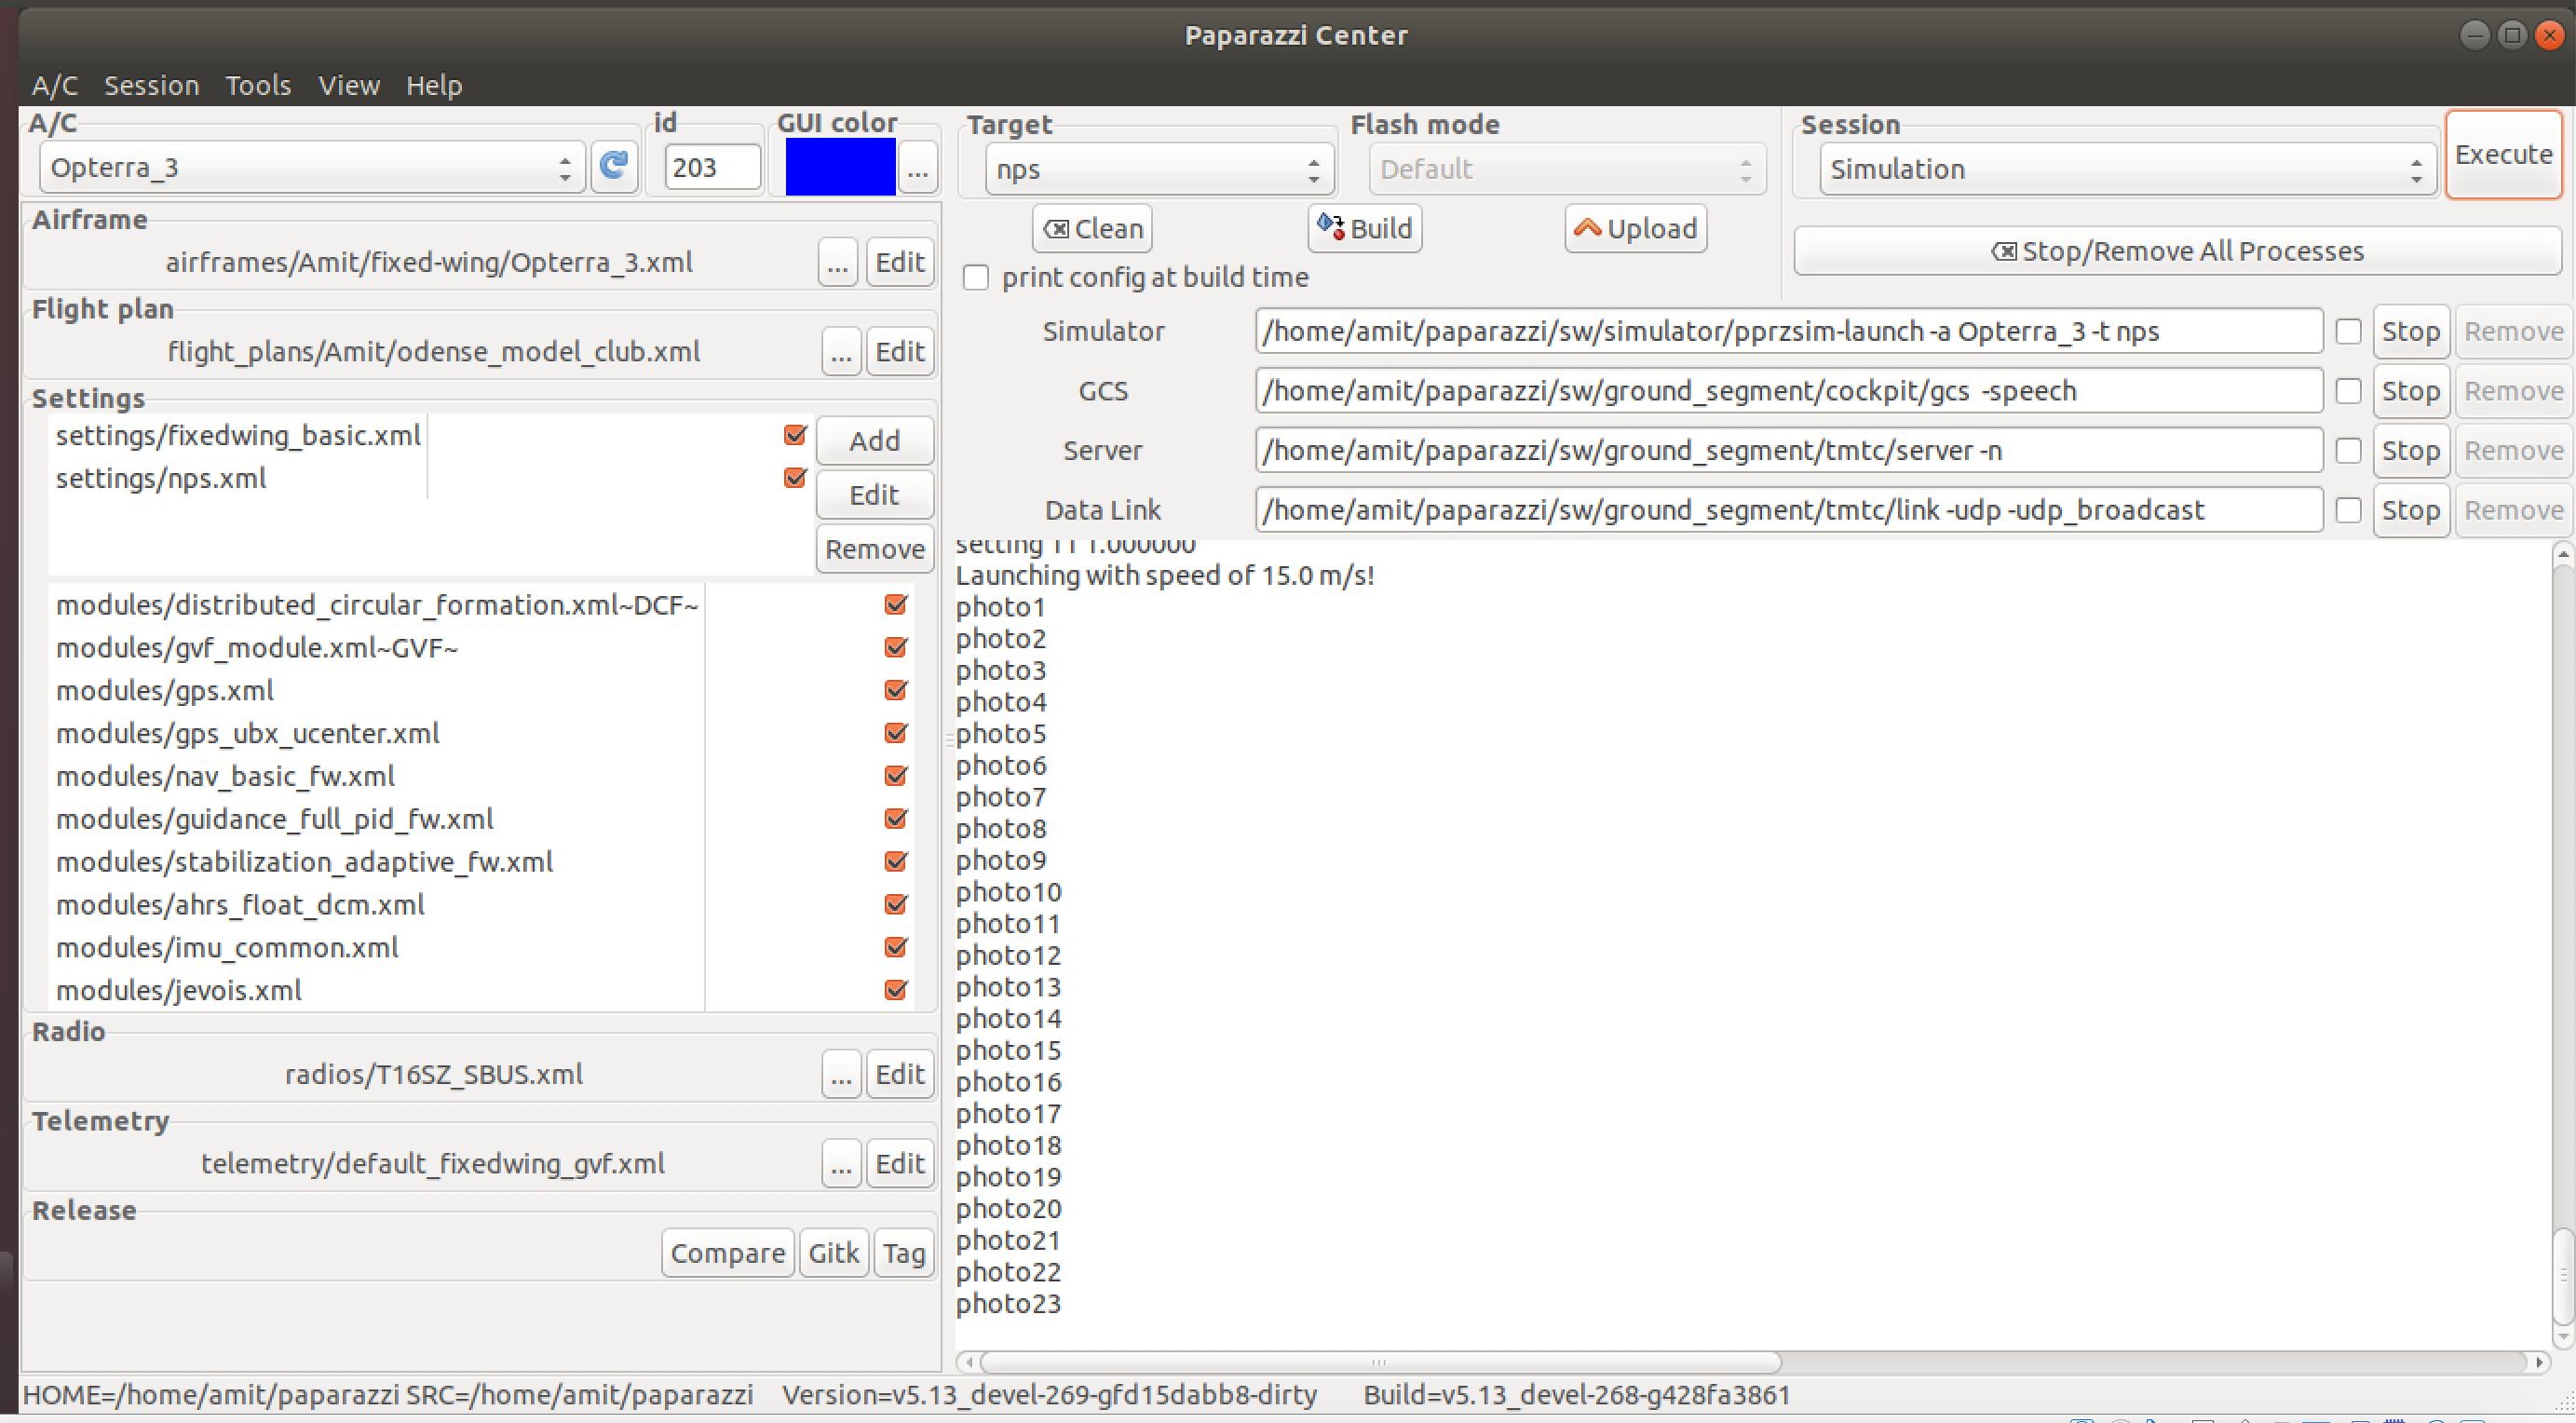
\includegraphics[width=10cm,height=10cm,keepaspectratio]{imagenes/Photos.png}
\caption{Photo capturing process simulation}
\label{fig:Photos}
\end{figure}